% Figure include snippets for the NLPCC 2026 draft.
% Prepared for later section-level integration; not automatically included.

% === Framework Figure: Selective Hybrid-Order Detector ===
\begin{figure}[t]
    \centering
    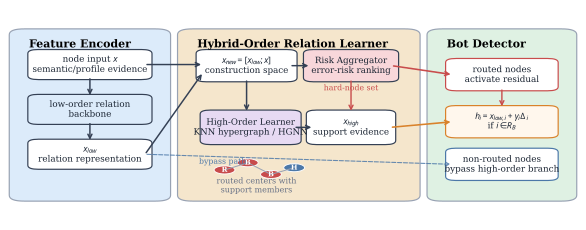
\includegraphics[width=\textwidth]{figures/Architecture_fit.pdf}
    \caption{Framework of the selective hybrid-order bot detector. The feature encoder produces node input and low-order relation representations; the hybrid-order relation learner uses a risk aggregator and a high-order learner to identify routed hard nodes and construct support evidence; the bot detector applies high-order residual correction only to routed nodes while non-routed nodes bypass the branch.}
    \label{fig:selective_hybrid_order_framework}
\end{figure}

% === Component Ablation Asset ===
\begin{figure}[t]
    \centering
    \includegraphics[width=0.92\textwidth]{figures/twibot20_component_ablation.pdf}
    \caption{Component ablation on TwiBot-20. The full model uses $K=8$, fanout 64, and a routed budget of 10\%.}
    \label{fig:twibot20_component_ablation}
\end{figure}

% === Hyperparameter Sensitivity Asset ===
\begin{figure}[t]
    \centering
    \includegraphics[width=0.92\textwidth]{figures/twibot20_seed1_hparam_sensitivity.pdf}
    \caption{Hyperparameter sensitivity on TwiBot-20. The dashed line and star marker indicate the full-model setting: $K=8$, fanout 64, and a routed budget of 10\%.}
    \label{fig:twibot20_hparam_sensitivity}
\end{figure}

% === Case Study Asset: BotUmc-Style Single Node ===
\begin{figure}[t]
    \centering
    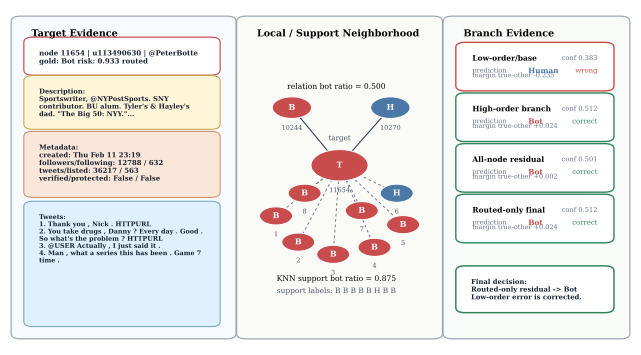
\includegraphics[width=\textwidth]{figures/casestudy.pdf}
    \caption{BotUmc-style case study for a routed hard node on TwiBot-20. The target account is misclassified by low-order evidence, while the high-order support set is bot-dominant and the routed-only residual branch corrects the final prediction.}
    \label{fig:casestudy}
\end{figure}
